\documentclass[11pt]{article}

% --------------------------------------------------
% Packages
% --------------------------------------------------
\usepackage[margin=1in]{geometry}
\usepackage{graphicx}
\usepackage{booktabs}
\usepackage{enumitem}
\usepackage{hyperref}
\usepackage{xcolor}
\usepackage{array}
\usepackage{tabularx}
\usepackage{amsmath}
\usepackage{enumitem}
\usepackage{xcolor}

% --------------------------------------------------
% Formatting
% --------------------------------------------------
\hypersetup{
    colorlinks=true,
    linkcolor=blue,
    citecolor=blue,
    urlcolor=blue
}

\setlength{\parskip}{0.5em}
\setlength{\parindent}{0pt}
\setlist[itemize]{leftmargin=1.5em}
\setlist[enumerate]{leftmargin=1.5em}

% --------------------------------------------------
% Project Information
% --------------------------------------------------
\newcommand{\coursename}{AI 360: Deep Learning}
\newcommand{\groupname}{JAE}
\newcommand{\projecttitle}{LaTeXWriting}
\newcommand{\blue}[1]{\textcolor{cyan!60!black}{#1}}

% --------------------------------------------------
% Document
% --------------------------------------------------
\begin{document}

\begin{center}
    {\Large \textbf{\coursename}}\\[0.4em]
    {\LARGE \textbf{Group Project Proposal}}\\[1em]
    {\large \projecttitle}\\[1em]
    \textbf{Group:} \groupname\\
\end{center}

Please describe your project in $\leq$4 pages excluding references.
This template is for guidance, and you can decide the exact details to include, but we do require you to complete each of the tables and we strongly suggest keeping each section that we have provided in the template.

\vspace{0.5em}
\hrule
\vspace{1em}

% ==================================================
\section{Group Composition}

\begin{center}
\begin{tabularx}{\textwidth}{l l}
    \toprule
    \textbf{Team Member} &
    \textbf{Student ID} \\
    \midrule
    \blue{Jordan Lieu} & \blue{33077652} \\
    \blue{Alex Yang} & \blue{52656155} \\
    \blue{Eddie Yang} & \blue{24738544} \\
    \bottomrule
\end{tabularx}
\end{center}

% ==================================================
\section{Introduction and Problem Definition}

Describe the problem that your project aims to address in 1 paragraph and
explain why it is interesting or important. Your introduction should address the following questions: \\\\
\blue{
In this project, we aim to solve the problem of translating handwritten mathematical expressions into a digital format, specifically \LaTeX{} code. As students, we often work through math problems on paper, and turning that work into a digital document means manually retyping every expression, which is slow and error-prone. We believe an automated solution could save considerable time and make mathematical work easier to share, edit, and submit. Because of the nature of handwriting where it varies, this project would be good for deep learning as it requires a model that can learn to recognize symbols across different writing styles, and it can also learn the syntax of \LaTeX{} itself. We therefore investigate whether, using existing training datasets and/or pretrained models, deep learning can convert handwritten mathematical expressions into accurate \LaTeX{} code.
}
% ==================================================
\section{Related Work and Background}
Briefly discuss relevant prior work, existing methods, and
approaches related to your problem. Identify the most relevant paper(s).

\begin{itemize}[noitemsep]
    \item How your proposed project relates to existing work.
    \item Which methods or ideas you intend to build upon.
\end{itemize}

\blue{
The modern approaches for handwriting recognition and latex translation problems use encoder-decoder methods.
Below is a list of papers we found that used encoder-decoder methods for related problems:
\begin{itemize}
    \item Im2Markup (2017): CNN + attention RNN, converting image straight to LaTeX.
    \begin{itemize}
        \item paper: https://proceedings.mlr.press/v70/deng17a.html
    \end{itemize}
    \item WAP (2017):  to handwriting. This is a classic baseline for handwriting recognition.
    \begin{itemize}
        \item paper: https://www.sciencedirect.com/science/article/abs/pii/S0031320317302376
    \end{itemize}
    \item BTTR (2021): switched to a Transformer decoder that reads left-to-right and right-to-left.
    \begin{itemize}
        \item paper: https://arxiv.org/abs/2105.02412
    \end{itemize}
    \item CoMER (2022): added coverage attention, which stops the model from skipping or repeating symbols.
    \textbf{This is the most relevant paper, and will likely be the idea we will build off of.}
    \begin{itemize}
        \item paper: https://arxiv.org/abs/2207.04410
    \end{itemize}
    \item Large OCR models (TrOCR, Nougat): powerful, but large and mostly trained on printed text.
    \begin{itemize}
        \item TrOCR paper: https://arxiv.org/abs/2109.10282
        \item Nougat paper: https://arxiv.org/abs/2308.13418
    \end{itemize}
\end{itemize}
}

\blue{
CoMER (Coverage information in a Transformer decoder for Mathematical Expression Recognition) is paper by Wenqi Zhao and Liangcai Gao. It takes an image of handwritten math
and outputs a LaTeX string, one token at a time.
}

\blue{
This is the exact same problem that we will try to be solving. However, instead of a CNN encoder, we'll be experimenting with a hybrid CNN + Transformer encoder.
 We'll also be using a Transformer decoder. Evaluation would be done on the CROHME benchmarks so results compare directly with published work.
}

% ==================================================
\section{Datasets}

Describe the datasets you plan to use for training, validation,
and testing. Specify:
\begin{itemize}[noitemsep]
    \item Dataset name and source (include a URL or citation).
    \item Task and type of data (e.g., images, video, text, or multimodal).
    \item Approximate dataset size and relevant characteristics.
    \item Intended training, validation, and test splits.
    \item Any preprocessing or data augmentation required.
    \item Access restrictions, licensing, or computational considerations.
\end{itemize}

Explain why the selected datasets are appropriate for the problem.

\blue{
\textbf{Datasets:} Below are the main datasets we will be using. Both datasets are perfectly aligned with our task: handwritten math paired with LaTeX.
Licensing for both is free for research as well. The dataset should be a few GB once rendered, and computation shouldn't take more than a day according to a quick google search.
}

\blue{
  \textbf{CROHME (handwriting competition benchmark) (https://zenodo.org/records/8428035)}
\begin{itemize}
    \item Handwritten strokes (InkML) plus LaTeX labels, rendered to images.
    \item About 9k expressions. Test sets: 2014 (\text{\textasciitilde1k}), 2016 (\text{\textasciitilde1.1k}), 2019 (\text{\textasciitilde1.2k}).
    \item Why: it’s the standard benchmark, so we can compare directly with CoMER and the other papers. It is also readily prepared for our specific task.
\end{itemize}
}

\blue{
\textbf{MathWriting (https://github.com/google-research/google-research/tree/master/mathwriting)}
\begin{itemize}
    \item Handwritten strokes plus LaTeX.
    \item About 230k real plus about 400k synthetic expressions, with official train/val/test splits.
    \item Why: about 25× bigger than CROHME, so less overfitting and room to test how much more data helps.
\end{itemize}
}

\blue{
\textbf{Split}: We will train on the MathWriting training split and use its validation split for model selection.
We will evaluate on the MathWriting test split and on the CROHME 2014, 2016 and 2019 test sets, which are the standard
benchmarks used in prior work. MathWriting provides substantially more training data than CROHME, which reduces
overfitting, while evaluating on CROHME allows direct comparison with published results. Because the CROHME test
sets are never used for training or model selection, and come from a different dataset with different writers,
they can be used to test generalization of our model nicely.
}

\blue{
\textbf{Preprocessing and Augmentation:}
There will be some preprocessing required for the dataset. We will need to render strokes to grayscale images and resize to a fixed height, clean up the LaTeX labels so equivalent formulas are written the same way, split the LaTeX into tokens like \texttt{\detokenize{\frac, \{, x, ^}}, and likely drop extremely long samples to fit GPU memory. For augmentations, we will add small rotations, scaling, stretching, distortion.
}

% ==================================================
\section{Available Hardware and Computational Resources}

Describe the computational resources available to your group. Include relevant details such as GPUs or other accelerators available (model and memory, if known) beyond colab if any.

\blue{
    NVIDIA 5070 RTX on local PC
}

% ==================================================
\section{Proposed Model and Methodology}

Describe your initial technical approach (this need not be a full definition of the model) and explain how you intend
to develop and evaluate your deep learning solution.

{\bf Model and Starting Point.}
Specify the model or architecture (e.g., CNN, RNN, GNN, etc.) you intend to use and justify your choice. Clarify the starting point of your project:
\begin{itemize}[noitemsep]
    \item Will you use an existing pre-trained model?
    \item Will you fine-tune an existing model on your task?
    \item Will you train a model from scratch?
    \item Will you adapt or combine existing architectures?
\end{itemize}

% Wenqi Zhao and Liangcai Gao in an ECCV 2022 paper
\blue{Given the nature of this problem, recognizing the expressions in images
and generating a sequence of latex tokens for each handwritten expression, we
plan to fine-tune the CoMER model mentioned in section 3.}

{\bf Proposed Approach.}
Outline the main steps of your proposed method (As much as possible at this stage), including:
\begin{itemize} [noitemsep]
    \item Input representation and preprocessing.
    \item Model architecture and key components.
    \item Training objective or loss function, if applicable.
    \item Optimization strategy and important hyperparameters.
    \item Inference procedure and expected outputs.
\end{itemize}
\blue{
  Steps:
  \begin{itemize}
    \item \textbf{Input representation and Preprocessing}: The handwritten
      strokes in MathWriting dataset are represented with Ink Markup Language
      (InkML), so they must be rendered into images before used for the
      training of the model.
    \item \textbf{Model architecture}: The architecture of CoMER is shown below.
      The two key components of the model are the DenseNet encoder, used to
      extract features from the rendered images, and the transformer to decode
      and generate the output. The fine-tuning starts from the head (linear \&
      softmax) layer and possibly improves FFN from CoMER.
      \begin{center}
          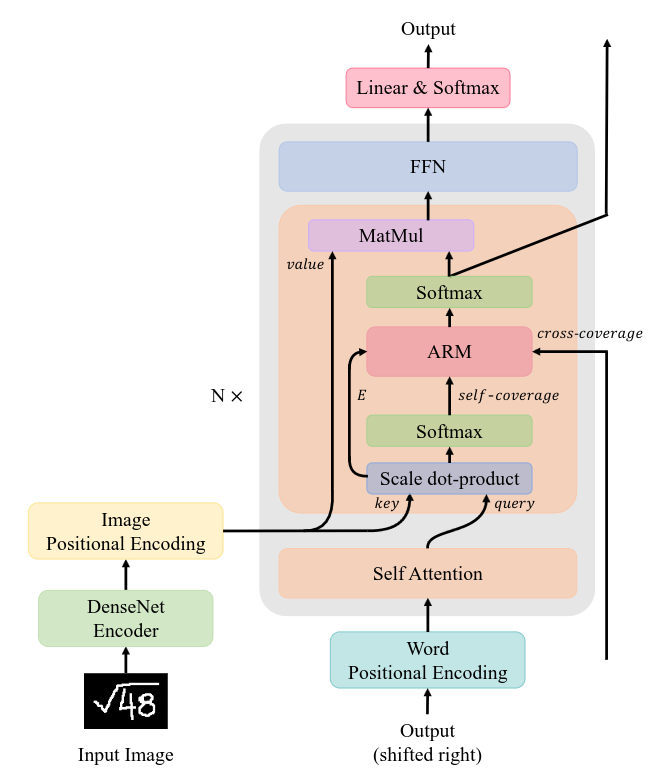
\includegraphics[width=0.50\textwidth]{CoMER-architecture.png} \\
      \end{center}
    \item \textbf{Optimization and hyperparameters}: We will use the same set of
      hyperparameters as the original CoMER model.
    \item \textbf{Expected Outputs and Inference Procedure}: The expected
      outputs are latex code sequences representing the handwritten expressions.
  \end{itemize}
}

We want you to provide enough detail to establish that the approach is technically plausible, while recognizing that the implementation and design may evolve.

{\bf Baselines and Evaluation.}

Describe how you will determine whether your approach is successful. Specify:
\begin{itemize}[noitemsep]
    \item Baseline methods or reference models.
    \item Evaluation metrics appropriate to the task.
    \item Experimental comparisons or ablation studies.
    \item Expected results and how they will be interpreted.
\end{itemize}
\blue{
  To evaluate the performance of our fine-tuned model, we will use CoMER as the
  reference and the metrics and official evaluation tool by the CROHME
  organizers, same as how designer of CoMER evaluated their model. We will also
  compare our fine-tuned model with other previously proposed solutions covered
  in section 3.
}

% ==================================================
\section{Timeline and Deliverables}

Provide a realistic timeline for the project, identifying milestones,
deliverables, and dependencies.

\begin{center}
\begin{tabularx}{\textwidth}{p{0.17\textwidth} X X}
    \toprule
    \textbf{Time Period} &
    \textbf{Milestone / Activities} &
    \textbf{Expected Deliverable} \\
    \midrule
    Week 1 & \blue{Lit. review and problem refinement} & \blue{Finalized problem and plan} \\
    Week 2 & \blue{Dataset preprocessing and pre-trained surgery} & \blue{Working data pipeline} \\
    Week 3 & \blue{Model development and training} & \blue{Initial model results} \\
    Week 4 & \blue{Fine-tuning} & \blue{Fine-tuned results} \\
    Week 5 & \blue{Final results and report} & \blue{Final report and slides} \\
    \bottomrule
\end{tabularx}
\end{center}

Adapt the timeline to the actual course schedule. Identify at least
one intermediate milestone that can be used to assess feasibility
and revise the approach if necessary.

% ==================================================
\section{Division of Work}

Describe the planned responsibilities of each team member. Explain how team members will coordinate and integrate their work.
Ensure that the distribution of work is clear and reasonably balanced.

\begin{center}
\begin{tabularx}{\textwidth}{l X X}
    \toprule
    \textbf{Team Member} &
    \textbf{Primary Responsibilities} &
    \textbf{Expected Contributions} \\
    \midrule
    \blue{Jordan, Alex, Eddie} & Literature review and problem formulation & Related work and project design \\
    \blue{Jordan} & Dataset preparation and preprocessing & Data pipeline and analysis \\
    \blue{Eddie} & Model implementation and training & Model and training code \\
    \blue{Alex} & Evaluation and experimental analysis & Metrics, comparisons, and visualization \\
    \bottomrule
\end{tabularx}
\end{center}


% ==================================================


\bibliographystyle{plain}
\bibliography{references}

% Alternatively, references can be listed manually using
% thebibliography if a separate .bib file is not used.

\end{document}
